\documentclass[12pt, letterpaper]{article}
\usepackage[utf8]{inputenc}
\usepackage[margin=0.75in]{geometry}
\usepackage{amsmath, amssymb}
\usepackage{titlesec, enumitem}
\usepackage{graphicx}
\usepackage{caption}
\usepackage{float}
\setlength\parindent{0pt}
\title{Minimax Quiz Questions}
\author{Team Chairun}
\date{November 29, 2020}

\begin{document}

\maketitle

1. Suppose we have the following payoff matrix for $A$ in a zero-sum game where $A$ moves first: \\
\begin{table}[H]
\centering
\begin{tabular}{|c|c|c|}
    \hline
    & $B$ Cooperates & $B$ Defects \\
    \hline
    $A$ Cooperates & -1 & 4 \\
    \hline
    $A$ Defects & 2 & 2 \\
    \hline
\end{tabular} \\
\end{table}
Assuming both players play optimally, what is $A$'s optimal strategy and payoff? \\

2. What is the purpose of using a heuristic in minimax? \\

3. Suppose a game where each player takes 2 turns in a row. How would the minimax algorithm change? \\

4. In the Tactics Solver assignment, there are some situations where the engine is unable to find the solution without a very high depth, regardless of the depth of quiescence search. What kind of situations might cause this? \\

5. Why would iterative deepening be used instead of breadth-first search in minimax? \\

6. Why can't we just search at a fixed depth until our alotted time runs out instead of using iterative deepening? \\

7. Fill in the node values calculated by minimax in the tree below and cross out branches pruned by alpha-beta pruning. $\Delta$ are maximizing and $\nabla$ are minimizing.
\begin{figure}[H]
    \centering
    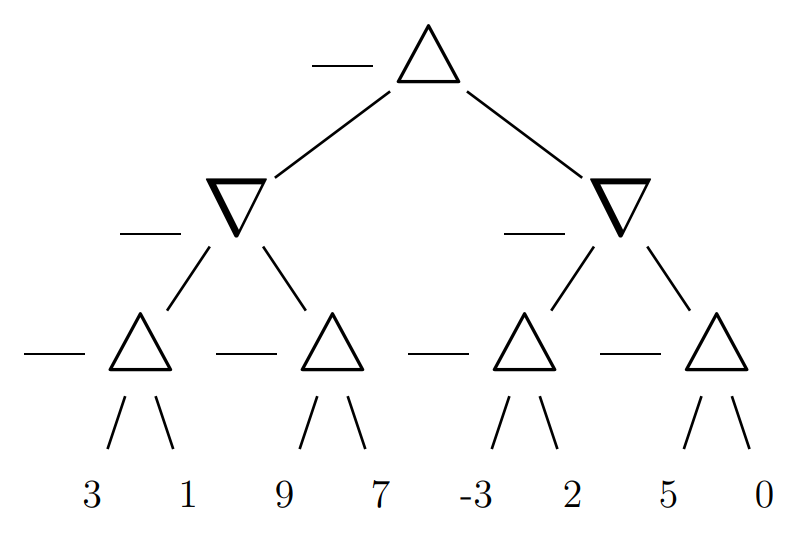
\includegraphics[scale=0.3]{minimax-prob.png}
    \caption*{From CS 61B Fall 2016 Midterm 2}
\end{figure}

8. Fill in values for $a$ and $b$ so that the crossed out branches shown below would be pruned by alpha-beta pruning.
\begin{figure}[H]
    \centering
    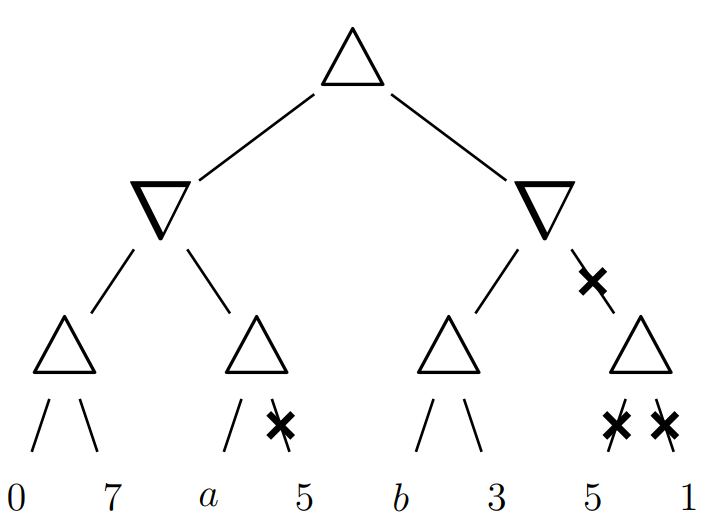
\includegraphics[scale=0.3]{alpha-beta-prob.png}
    \caption*{From CS 61B Fall 2016 Midterm 2}
\end{figure}


9. Suppose you have the functions findMax and findMin as written in the slides. You wish to find the best move for a game, but for some reason the heuristic you have gives payoffs which are flipped. How do you find the best move for the player which normally would be maximizing? \\

10. In chess, there are positions which are referred to as "sharp," where the position is volatile and the evaluation can change very drastically depending on the moves played. Would alpha-beta pruning run more quickly in a "sharp" position or a non-"sharp" position relative to conventional minimax with no pruning? \\

11. Suppose a game with a branching factor of 7. How many states do we search if we begin a minimax search with no pruning of depth 3? \\

12. Explain possible drawbacks to the following heuristic for the board game Connect-4, where the goal is to get $4$ pieces in a row: $(\text{Reds in a row}) - (\text{Blacks in a row})$.

13. Explain why in a transposition table we store not just an evaluation of a state, but the depth of that evaluation as well. \\

14. What are some ways that we can choose good moves for move ordering? \\

15. Explain how quiescence search is able to mitigate some of the effects of the horizon effect.\\
\end{document}
\end{document}